\section{Beispiele}

Dies ist Platzhaltertext für die Diskussion der Resultate. Hier werden die in
Kapitel~\ref{sec:resultate} vorgestellten Ergebnisse eingeordnet und kritisch bewertet.

\subsection{Beispiel für Querverweise}
\label{subsec:querverweise}
Mit dem Paket \texttt{cleveref} können Querverweise automatisch mit dem passenden Typ
beschriftet werden, zum Beispiel ein Verweis auf \Cref{tab:beispieltabelle} oder auf
\Cref{fig:beispielbild}. Ebenso kann erneut auf eine Quelle verwiesen werden
\cite{muster_beispielquelle_2025}.

\subsection{Einschränkungen}
\label{subsec:einschraenkungen}
Dies ist Platzhaltertext für die Beschreibung von Einschränkungen oder offenen Fragen.


\subsection{Beispiel mit farbig hervorgehobener Tabelle}
\label{subsec:beispiel-farbtabelle}
Mit dem Paket \texttt{xcolor} (Option \texttt{table}) können einzelne Tabellenzeilen
hervorgehoben werden, siehe Tabelle~\ref{tab:beispiel-farbtabelle}.

\begin{table}[h!]
    \centering
    \caption{Beispieltabelle mit farbig hervorgehobenen Zeilen.}
    \label{tab:beispiel-farbtabelle}
    \begin{tabularx}{\textwidth}{l *{2}{>{\centering\arraybackslash}X}}
        \toprule
        \textbf{Punktnr.} & \textbf{Abweichung [cm]} & \textbf{Bemerkung} \\
        \midrule
        1001 & 1.2 & Platzhalter \\
        \rowcolor{lightgray}
        1002 & 3.4 & \textcolor{red}{\textbf{Auffälliger Wert}} \\
        1003 & 0.8 & Platzhalter \\
        \bottomrule
    \end{tabularx}
\end{table}

\subsection{Beispiel einer mehrspaltigen Liste}
\label{subsec:beispiel-multicol}
Mit dem Paket \texttt{multicol} können Aufzählungen auf mehrere Spalten verteilt werden,
zum Beispiel für Listen mit vielen kurzen Einträgen: \todo{Dies ist ein To-do Kommentar}

\begin{multicols}{2}
    \begin{itemize}
        \item Eintrag 1
        \item Eintrag 2
        \item Eintrag 3
        \item Eintrag 4
        \item Eintrag 5
        \item Eintrag 6
    \end{itemize}
\end{multicols}

\subsection{Beispiel eines einfachen Diagramms}
\label{subsec:beispiel-tikz}
Mit dem Paket \texttt{tikz} können einfache Diagramme direkt in \LaTeX{} erstellt werden,
siehe \Cref{fig:beispiel-tikz}.

\begin{figure}[h!]
    \centering
    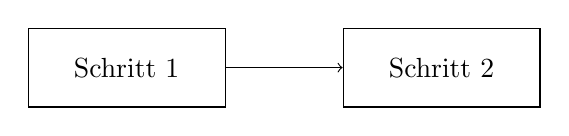
\begin{tikzpicture}
        \node[draw, rectangle, minimum width=2.5cm, minimum height=1cm] (a) at (0,0) {Schritt 1};
        \node[draw, rectangle, minimum width=2.5cm, minimum height=1cm] (b) at (4,0) {Schritt 2};
        \draw[->] (a) -- (b);
    \end{tikzpicture}
    \caption{Beispiel für ein einfaches \texttt{tikz}-Diagramm.}
    \label{fig:beispiel-tikz}
\end{figure}

\FloatBarrier


\subsection{Zielsetzung}
Dies ist eine Aufzählung:
\begin{itemize}
    \item 1 Punkt.
    \item 2 Punkt.
    \item ...
\end{itemize}


\subsection{Vorgehen}
\label{subsec:vorgehen}
Dies ist Platzhaltertext zur Beschreibung des methodischen Vorgehens. Hier werden die
einzelnen Arbeitsschritte erläutert.

\begin{tcolorbox}[myboxstyle, title=Hinweis]
Dies ist eine Beispiel-Hinweisbox (\texttt{tcolorbox}). Sie eignet sich, um wichtige
Hinweise, Annahmen oder Einschränkungen hervorzuheben.
\end{tcolorbox}

\subsection{Beispielrechnung}
\label{subsec:beispielrechnung}
Formeln können mit \texttt{amsmath} gesetzt werden, zum Beispiel die Berechnung einer
Bodenauflösung (GSD) in Abhängigkeit der Flughöhe:
\begin{equation}
    \text{GSD} = \frac{h \cdot p}{f}
    \label{eq:gsd}
\end{equation}
mit Flughöhe $h$, Pixelgrösse $p$ und Kamerakonstante $f$. Mit dem Paket \texttt{siunitx}
können Einheiten konsistent gesetzt werden, zum Beispiel eine Flughöhe von \SI{60}{\meter}.
Gleichung~\ref{eq:gsd} bzw.\ \cref{eq:gsd} kann so im Text referenziert werden.

\subsection{Beispieltabelle}
\label{subsec:beispieltabelle}
Tabelle~\ref{tab:beispieltabelle} zeigt den Aufbau einer Beispieltabelle mit
\texttt{tabularx}, \texttt{threeparttable}, \texttt{multirow} und \texttt{makecell}.

\begin{table}[h!]
    \centering
    \caption{Kontrollmessungen zur Bestimmung des Fehlers aus den Basisdaten.}
    \label{tab:beispieltabelle}
    \begin{tabularx}{\textwidth}{c | *{3}{>{\centering\arraybackslash}X}}
        \toprule
        \makecell{\textbf{Höhe} \\ \textbf{[m.ü.M]}} & 
        \makecell{$\mathbf{\Delta E_{VRS} - E_{MDR}}$ \\ \textbf{[cm]}} & 
        \makecell{$\mathbf{\Delta N_{VRS} - N_{MDR}}$ \\ \textbf{[cm]}} & 
        \makecell{$\mathbf{\Delta H_{VRS} - H_{MDR}}$ \\ \textbf{[cm]}} \\
        \midrule
        1885 (Fix 1) & -2.1 & 0.8 & \textcolor{red}{\textbf{5.5}} \\
        1885 (Fix 2) & -2.6 & 1.8 & \textcolor{red}{\textbf{5.2}} \\
        2085 & -0.6 & -2.5 & \textcolor{red}{\textbf{3.6}} \\
        2145 & -0.7 & -2.9 & \textcolor{red}{\textbf{5.9}} \\
        2205 & -0.5 & -2.4 & \textcolor{red}{\textbf{5.1}} \\
        2255 & -1.1 & -2.1 & \textcolor{red}{\textbf{4.6}} \\
        \midrule
        \textbf{} & 
        $\mathbf{RMSE_E}$ \textbf{[cm]} & 
        $\mathbf{RMSE_N}$ \textbf{[cm]} & 
        $\mathbf{RMSE_H}$ \textbf{[cm]} \\
        \midrule
        \textbf{} & 0.9 & 2.4 & \textcolor{red}{\textbf{5.0}} \\
        \bottomrule
    \end{tabularx}
\end{table}

\subsection{Beispielabbildung}
\label{subsec:beispielabbildung}
\Cref{fig:beispielbild} zeigt eine Beispielabbildung inklusive Bildlegende und Quellenangabe.

\begin{figure}[h!]
    \centering
    
\includegraphics[width=\textwidth]{aufnahmeperimeter_Skipiste1.jpg}
    \caption[Beispielabbildung zur Illustration des Bild- und Beschriftungsformats]{Beispielabbildung zur Illustration des Bild- und Beschriftungsformats.
    \\Projektion:~LV95~|~Stand:~TT.MM.JJJJ~|~Datenquelle:~Platzhalter}
    \label{fig:beispielbild}
\end{figure}

\FloatBarrier
